\documentclass{llncs}
\pagestyle{headings}   % turn on page numbers
\usepackage{epsf}
\usepackage{epsfig}

\usepackage{url}

\newcommand{\Circus}{{\sf\slshape Circus}}
\newcommand{\Class}[1]{\texttt{#1}}
\newcommand{\Element}[1]{\texttt{#1}}
\newcommand{\Interface}[1]{\texttt{#1}}
\newcommand{\Method}[1]{\texttt{#1}}

\begin{document}
\title{CZT Support for Z Extensions}
\author{Leo Freitas$^1$ \and Tim Miller$^2$ \and Petra Malik$^3$ \and Mark Utting$^3$}

\institute{%
   \begin{tabular}{cc}
      University of York, UK  $\quad\quad$ & University of Liverpool, UK
      \\ %
      $^1$\texttt{leo@cs.york.ac.uk} $\quad\quad$ & $^2$\texttt{tim@csc.liv.ac.uk}
   \end{tabular}
   \begin{tabular}{c}
      University of Waikato, New Zeland
      \\ %
       $^3$\texttt{\{petra, marku\}@cs.waikato.ac.nz}
   \end{tabular}
} %

\maketitle


\begin{abstract}
  The Community Z Tools (CZT) is an integrated framework for supporting the Z formal notation
  and its multiple extensions. Through extensible design patterns it considerably improves
  code reuse, maintainability, debugging, and so on.
  The main facilities provided are parsing, typechecking, and an interchangeable markup format
  that conforms with the Z ISO standard. This markup format accepts inputs such as \LaTeX,
  Unicode, and e-mail. Furthermore, other facilities like animation, persistence, and automated
  GUI building are also available.
  The available Z extensions are present across all these facilities, hence showing the
  usefulness of such an integrated framework.

  \noindent
  \textbf{Keywords}: Standard Z, Object-Z, \Circus, TCOZ, design patterns, parsing, typechecking, animation.

\end{abstract}

\section{Introduction} \label{sec:intro}

  The Z language~\cite{isoz} is a formal specification notation that
  can be used to precisely specify the behaviour of systems, and
  analyse it via proof, animation, test generation, and so on.  The Community
  Z Tools (CZT) project~\cite{czt} is an open-source Java framework
  for building formal methods tools for Z and Z extensions.

  In recent years, there has been an increasing interest in combining
  different programming paradigms within an uniform formal notation,
  where Z plays a central role. This gave rise to many Z extensions that
  includes process algebras~\cite{fischer-1998,fischer-2000,circus.sem:intro},
  object orientation~\cite{oz,ohcircus}, time~\cite{tcoz,circus.sem:real.time2},
  mobility~\cite{circus.sem:mobility}, and so forth.

  Among these extensions, CZT supports Object-Z~\cite{oz}, a
  specification language that extends Z with modularity and reuse
  constructs that resemble the object-oriented programming
  paradigm. Such constructs include classes, inheritance, and
  polymorphism. CZT supports Object-Z in the form of parsing,
  typechecking, and other facilities.  Currently, we are working on
  extensions for Timed Communicating Object-Z (TCOZ)~\cite{tcoz},
  which is a blend of Object-Z and Timed-CSP~\cite{timed-csp}, as well
  as extensions for \Circus~\cite{circus.sem:intro}, a unified
  refinement language that combines Z, CSP~\cite{csp.books:roscoe},
  and the refinement calculus~\cite{fm.ref:morgan}, with Hoare and
  He's \textit{Unifying Theories of Programming} (UTP) as the semantic
  background~\cite{hoare.utp}.

  In CZT, we aim to provide tool support for all of these extensions,
  while maximising the commonality between the languages, and
  minimising versioning and maintenance. This paper presents a
  framework for doing so using many different techniques, each suited
  to the type of tool that is being implemented. {\bf This paragraph is
  not quite there!!}

  In Section~\ref{xml-schemas}, we present a method for specifying an
  XML interchange format that maximises commonality, while
  Section~\ref{java-ast-classes} presents the generation of
  \emph{Annotated Syntax Tree} (AST) classes from this XML
  documentation. Section~\ref{parsers} presents a method for
  generating parsers, scanners, and other related tools for the
  different the Z extensions, and Section~\ref{typecheckers} presents
  the design of the CZT typecheckers, which are tailored for
  extendability and reuse. Section~\ref{animation} presents the
  animation method used in the CZT animator, ZLive, and discusses the
  possibility of using this to animate extensions to
  Z. Section~\ref{section-manager} presents the design of the {\em
  section manager}, an integral component of CZT that caches
  information about specifications to improve the efficiency of the
  tools, while Section~\ref{other-tools} briefly discusses other CZT
  tools. Section~\ref{sec:conclusions} concludes the paper and
  discusses the future of the CZT project.


\section{XML Schemas}
\label{xml-schemas}

  The first step in designing the CZT tools and libraries was the
  development of an XML Schema that describes an XML markup for Z
  specifications (ZML)~\cite{UttEA:03}.  This is an interchange format
  that can be used to exchange parsed and even typechecked Z
  specifications between sessions and tools.

  The idea of using Z with XML has also been explored in the
  Z/Eves theorem prover~\cite{tp.tools:zeves.ref}. It allowed one to
  create a customised theorem prover with additional tactics tailored
  for a particular specification by modifying the XML representation
  of the Z specification in Z/Eves~\cite{tp.tools:zeves.api}.
  The main problem however, was the lack of a common standard.
  The effort indeed pointed to an appropriate direction tough.

  Standard Z allows specifications to be exchanged using Unicode,
  \LaTeX\ or email markup.  However, implementing a parser for such
  specifications is a non-trivial task that might take several weeks
  or even months to be finished.  ZML, in contrast, can be parsed
  immediately using one of the available XML parsers like
  Xerces\footnote{\url{http://xml.apache.org/xerces-j/}} or
  Crimson\footnote{\url{http://xml.apache.org/crimson/}}.

  Tools also benefit from being able to annotate terms with type
  information, anticipated usage, comments, location, and so on.
  The ZML format allows such annotations. [TODO: are there other advantages of ZML?]

  The XML Schema for ZML has been carefully designed to be extensible
  in order to allow Z extensions to profit from those advantages as well.
  The following strategies have been used to achieve this.

  The \textit{``any''} element can be used in an XML Schema to enable
  instance XML documents to contain additional elements not specified
  by the schema.  This concept has been used to define annotations.
  That is, an annotation to a term can either be one of the
  annotations defined in the XML Schema for Z, or any other kind of
  data.  This allows a tool builder to decide what data makes sense
  for a particular tool.

  Secondly, inheritance is used extensively throughout the XML Schema.
  Abstract elements are used to provide placeholders for their derived
  elements.  For example, the abstract element \Element{Para} is the
  parent of all concrete Z paragraphs like, for example, axiomatic
  paragraphs (element \Element{AxPara}), and free types paragraph
  (element \Element{FreePara}).  This makes it easy to include a
  reference to any kind of paragraph into other elements as, for
  example, in the definition of a Z section (element \Element{ZSect})
  which contains a sequence of paragraphs.

  More important is, however, that the inheritance hierarchy defined
  in the XML Schema for ZML can be extended without even touching the
  ZML Schema file.  For example, the XML Schema for Object-Z imports
  the ZML Schema file and defines a new paragraph for classes (element
  \Element{ClassPara}) that is derived from element \Element{Para}
  defined in the ZML Schema.  Instance documents of the Object-Z
  Schema can now contain class paragraphs in addition to the Z
  paragraphs wherever a paragraph is expected.  The same strategy has
  been used to define expression (abstract element \Element{Expr}),
  predicates (abstract element \Element{Pred}), declaration (abstract
  element \Element{Decl}) and others, making it possible for
  extensions to add new kinds of expressions, predicates, etc.

  This can be carried on to extending an extension.  For example, the
  additional elements provided by the Object-Z Schema are further
  extended by the TCOZ Schema.  Again, the definitions of the elements
  for TCOZ are encapsulated into a TCOZ Schema file, and the ZML or
  Object-Z Schema do not need to be modified.
  Similarly, the \Circus\ extension for CZT is encapsulated into a
  \Circus\ XML schema file that extends the main standard Z schema.
  This approach of extension via inclusion is explored throughout the
  different layers of CZT tools.
  The resulting net effect is that once one package is finished, it
  can be directly extended through inheritance, hence simplifying the
  task of extending standard Z in a great extent.

  [TODO: are there other things that make the Schema extensible?]

  The use of XML in the CZT has shown as an efficient and extensible
  solution for representing a Z specification and its extensions.  The
  XML approach helps to clarify design decisions in a straightforward
  fashion.  This representation is the key for the integrated
  development and exchange of information among different Z tools.

\section{Java AST Classes}\label{java-ast-classes}

  The Java \emph{Annotated Syntax Tree} (AST) provides a tree view of
  a parsed specification using Java interfaces and classes.  This
  allows easy access to syntactical objects like, for instance,
  paragraphs, declarations, predicates, and expressions, from within
  Java programs.

  The CZT Java AST interfaces and classes were automatically generated
  from the XML Schemas described in the previous section using our
  code generator \emph{GnAST} (GeNerator for AST).  The generated code
  looks similar to the code Java data binding tools like
  JAXB\footnote{\url{http://java.sun.com/xml/jaxb/}} or
  Castor\footnote{\url{http://www.castor.org/}} are producing.  The
  generated Java interfaces and classes represent the structures
  defined in the XML Schema instance document.  While the main purpose
  of a Java binding tool is to provide the ability to convert from XML
  format to Java objects and vice versa, the main purpose of GnAST is
  to generate well-designed AST classes.  For example, the AST classes
  generated by GnAST support the visitor design pattern described
  later on.

  The automatic AST generation from the XML schemas alone is already a
  considerable improvement in productivity and maintainability.  For
  instance, the complete AST folder representing standard Z contains
  around $420$ Java files.  GnAST has also been used to generate AST
  interfaces and classes for Object-Z, TCOZ, and \Circus.  In total,
  from the four XML schema files Z and its extensions, GnAST
  automatically generates around $2300$ Java files.  This provides a
  very convenient way to obtain AST's for Z extensions that fit well
  into the AST for standard Z.  That is, the AST classes for Z
  extensions also support ZML as well as the visitor design pattern
  described below.

  The visitor design pattern~\cite{GamEA:95,MaiCha:01} makes it very
  easy to write tools like typecheckers and printers, that need to
  traverse an AST. It provides a way to separate the structure of a
  set of objects from the operations performed on these objects.  This
  allows both a new operation to be defined without modifying the AST
  classes, and vice-versa.  To define a new operation, all you need to do is
  to implement a new visitor class.

  [LEO: I think the last part of this paragraph needs more review for
  clarity.  {\bf Petra:} I agree.  I am still not sure how much
  description of the visitor design patter is needed.  It has been
  introduced in the ZB paper, so we could refer to this paper, having
  something like a summary here.  Or we could copy the description
  from there (about two or three pages) and revise it.  Any thoughts?]

  In CZT, a visitor interface is defined for every AST class,
  including abstract superclasses.  So, if a visitor implements an
  interface, say \Interface{AxPara}, then any \Interface{AxPara} AST
  nodes that it visits will call the visitor's \Method{visitAxPara}
  method.  However, if the visitor does not implement the
  \Interface{AxParaVisitor} interface, then the \Interface{AxPara} AST
  nodes will search up though their superclasses and call the first
  \Method{visit$AAA$} method that the visitor implements. For example,
  \Interface{visitPara}, \Interface{visitTermA} or \Interface{visitTerm},
  the superclasses of \Interface{AxPara}.
  With this approach, the AST classes themselves take care of calling
  the closest (with respect to the inheritance hierarchy)
  \Method{visit} method implemented by the visitor.

  This flexibility and independency of visitors is very useful during
  the development of new tools.  As the hierarchy trees of different
  language entities are independent, one can implement visiting
  methods for specific parts of the language such as declarations or
  paragraphs.  That allows one to implement the hierarchy trees
  piecemeal, checking the conformance within every stable subset.
  Whenever problems are found, they are contained within the visit
  methods for the particular hierarchy tree, hence improving debugging
  and maintainability.  For instance, in the development of the
  \Circus\ compiler used in a model checking
  tool~\cite{circus.mc:leo}, the use of CZT visitors allowed the
  implementation of the smallest subset needed for initial testing.
  This makes the CZT visitor not only an elegant object oriented
  solution, but also the ground for consistent rapid prototyping.

\section{Parsers, Scanners, and Related Tools}
\label{parsers}

  CZT includes a suite of important tools for operations such as
  parsing, typechecking, and markup conversion. In addition to a
  parser and typechecker for Z, an Object-Z parser is provided, and
  \Circus\ and TCOZ parsers, as well as Object-Z and \Circus\
  typecheckers, are under development.  The Object-Z, TCOZ, and
  \Circus\ tools extend the Z tools by adding support for the
  additional constructs these languages provide.  Each language is an
  extension of Z, so it is tempting to just keep adding to the tools
  for each extension and use the largest superset of all extensions. For
  example, use the TCOZ tools to parse and typecheck Z. However, this
  has two distinct problems. Firstly, one aim of the CZT project is to
  create tools that strongly conform to the Z standard, so allowing
  extra constructs and different type-rules will break the strong
  conformance. Secondly, the extensions of Z are not linear. For
  example, Object-Z extends Z with class paragraphs, and TCOZ extends
  Object-Z with concurrency operators, but \Circus\ extends neither of
  these --- only Z. Therefore, CZT requires an approach that produces
  separate tools for each Z extension, maximises the commonality between
  the parsers, and minimises versioning and maintenance problems via
  reuse.


  \begin{itemize}
    \item[LEO] Ok. What do you think about the idea of hard-coded toolkits to
               improve performance that I've included in Section~\ref{multiple-markups}?
  \end{itemize}

\subsection{Parsers and Scanners}

  CZT includes parsers for standard Z specifications given either in
  Unicode or using \LaTeX\ markup.  Support for e-mail markup is
  planned. To produce different parsers and scanners for Z and its
  extensions, CZT uses XML templates, and generates the code from these
  templates using XSLT, a language for transforming XML. Java
  Cup\footnote{See
  \url{http://www.cs.princeton.edu/\~{}appel/modern/java/CUP/}} is
  used to generate the CZT parsers from an LALR grammar, and
  JFlex\footnote{See \url{http://jflex.de/}} is used to generate the
  scanners. 

  \begin{itemize}
    \item[Tim] I have moved this paragraph below from the opening
    paragraph of this section, because it is only related to parsers
    and scanners.
  \end{itemize}

  Unfortunately, it is quite difficult to reuse code from an
  automatically generated scanner or parser, and neither Java Cup nor
  JFlex explicitly supports inheritance for parser or scanners
  respectively.  To avoid duplicated code, XML templates that contain
  the different parser and scanner variants are used. From this, the
  different Java source files for each Z extension are generated using
  XML translation tools.  This maximises the commonality between the
  parsers and minimises versioning and maintenance problems.

The parser and scanner for all Z extensions are maintained in two
master XML files: one for the parser and one for the scanner. Each
master file contains several XML tags that are used for substituting
text for each Z extension. For example, the {\tt <package/>} tag is
placed wherever one would normally write the Java package name, so
that each parser and scanner can be contained in their own
package. The tags {\tt <add:}{\em extension}{\tt >} and {\tt </add:}{\em
extension}{\tt >} are used to wrap around code that are specific to
particular Z extensions. So to add a new type of expression to the
Object-Z parser, one would add a new production to the expression rule
in the master file, and place it between the {\tt <add:oz>} and {\tt
</add:oz>} tags, for example.

To generate the individual Java Cup files for each extension of Z,
XSLT is used to include the necessary code, and to substitute in
values for tags. For example, to generate the Object-Z parser, XSLT is
applied to the master file, and supplied with the three arguments
below:
\begin{enumerate}
  \item {\tt "class"} substituted with {\tt "Parser"}.
  \item {\tt "package"} substituted with {\tt "net.sourceforge.czt.parser.oz"}.
  \item {\tt "oz"} expressions to be included.
\end{enumerate}

Additional arguments including the input and output files are also
required.

Similar rules are specified for each Z extension. The result is a series
of Java Cup and JFlex files, one for each extension, which can then be
used to generate the parser and scanner code.

The use of XML templates enables parsing code to be reused and easily maintained.
Extending the framework for a new extension incurs in just adding the important
grammar and lexer rules together with few modifications such as those parameters above.
For example, we are experimenting the incorporation of the available \Circus\
parser~\cite{circus.other:parser} rules within the flexible CZT framework. The
obvious advantages are the widely tested and supported standard Z classes, \LaTeX\
markup and Unicode, visiting and other facilities.

\subsection{Multiple Markups}\label{multiple-markups}

 CZT supports multiple markups for each Z extension.  The different
 markup languages suit different communities.  For example, \LaTeX\
 is preferred by researchers while Unicode WYSIWYG editing might be
 more attractive for students or industrial users. At present,
 Unicode, \LaTeX, and the ZML format are supported~\cite{UttEA:03},
 but adding additional markups is straightforward, as this section
 will present.  ZML scanning will not be discussed here, because it is
 quite different to the other markups;~these can be found elsewhere~({\bf add a reference here}).
 For ZML, JAXB code ({\bf find a reference}) is used to covert the ZML into an abstract syntax tree.

The CZT parsers are markup independent, but all of our scanners will
provide their respective parsers with Unicode when scanning Z variable
names, for instance. The reason for this is straightforward: Z specifications
are made up of sections, with each section having a name and a list of
parent sections. The definitions in a parent section are included in
the child section for a specification. For example, the Z toolkit is
specified as a series of \LaTeX\ sections. Now, consider the case in
which a person would like to use the Z toolkit, but would like to use
Unicode for their own specifications. This would require CZT to
provide a Z toolkit in Unicode, because the names used for
declarations in the Z toolkit would be in \LaTeX~instead of
Unicode. To work around this problem, all markups are converted to
Unicode, therefore allowing different sections of a specification to
be written in different markups.
With this architecture, each Z extension can also provide its own
particular toolkit extension given as a \LaTeX\ specification file.
The extended toolkits usually contains keywords, special symbols,
and commonly used functionality described with standard Z templates, for instance.

Therefore, CZT provides a Unicode scanner, which performs lexical
analysis on a Unicode stream and breaks it into the necessary
tokens. CZT's \LaTeX~scanner, instead of implementing all of the
scanner rules, converts its \LaTeX~stream into a Unicode stream. In
addition to solving the problem discussed above, this greatly
simplifies the \LaTeX~scanner, because much of the conversion is
straightforward in comparison to scanning Z tokens. Moreover, location
information is recorded in the ASTs using annotations on each of the
nodes, and this points to the location in the original specification file.

Of course, the \LaTeX~to Unicode scanner needs to know how to convert
\LaTeX~tokens into Unicode. This is done by specifying, in the \LaTeX\ file,
the corresponding Unicode representation for each \LaTeX~token used. For example, in
the Z toolkit \LaTeX~file, the following rule is written specifying the \LaTeX~
token for powerset (\verb+\power+):
\begin{verbatim}
  %%Zprechar \power U+2119
\end{verbatim}
%
The {\tt \%\%Zprechar} keyword specifies that \verb+\power+ is a
prefix character that always has a hard space after it, and
that its Unicode equivalent is U+2119. There are similar operators for
postfix, infix, and nofix characters, as well as words.

An additional component parses these definitions, and records this in
a symbol table. Each time a \LaTeX~token is read, a lookup is
performed on this table to find the Unicode mapping. If the lookup
fails because the token is not in the table, a warning is issued, and
the \LaTeX~token is used, minus the \verb+\+ token at the
front. Therefore, for each new \LaTeX~token introduced into a
specification, a unique Unicode mapping must be provided for the
\LaTeX~to Unicode scanner, or be content with using the \LaTeX~token's
base name.

The price to pay for such flexibility is a slower parsing experience
whenever too complex markup is found.  We are currently working in
ways around this performance penalty.  One possible optimisation is to
have the option to use hard-coded versions of standard sections such
as the Z toolkit.  Since most Z section specifications do include the
Z toolkit, then this should improve parsing performance considerably
because no parsing will be necessary for the Z toolkit included as a
parent of other used-defined Z sections.  This notion can be
generalised for other Z extensions, provided their extended toolkits reach
an enabling level of stability.

To parse a specification written using a new markup, for example, the
e-mail text-based markup, one only has to implement an e-mail to Unicode
scanner. This approach has an additional advantage: the scanners can function as
converters between different markups without have to parse the
specifications. This simplifies many other tools in the suite as
well. For example, the CZT tool suite provides printing of abstract
syntax trees into the different markups. However, instead of
implementing a printer for each markup, only a Unicode printer is
implemented, and converters are used to print the other markups.

\subsection{Extending Tools using Visitors}
\label{extending-visitors}


\section{Typecheckers}
\label{typecheckers}

\begin{quotation}
[LEO: Comments at paragraphs from: ``To extend the Z typechecker,
      a new package is created.''

      \vspace{5pt}

      These paragraphs are too dense. They require (or presume) good knowledge of
      the underlying architecture. For example, the intrinsic relationship between
      individual checkers and the main typechecker class, or the unification environment.
      I suggest to change some of it, perhaps with a running example, so that it is easier
      for the naive reader to follow.
      Moreover, although I understand the argument for the unusual design,
      I think it ought to be strengthened. As it is, it does not sound convincing
      enough perhaps because of the text's density. The example with oz could be
      a good thing to come earlier, but it is far from clear.

      \vspace{5pt}

      Tim, what do you think? Does it make sense?
      I will include some text and rearrange text a little to (hope
      to) improve clarity.

      [Tim]: Leo, this is very good. I only hacked this up on Friday
      and hadn't read it at all, but these changes are very nice.

      Remark: on the code example given, the class {\tt oz.ExprVisitor} is mentioned.
      Don't you mean {\tt oz.ExprChecker}?

     [Tim]: Yes indeedly.

      Please, let me know what do you think, ok? So that I do not include any non-sense! :)
      I will also blend my experiences with the \Circus\ typechecker in the end.
      ]
\end{quotation}

Typecheckers in CZT are written in a much different way from the parsers
and scanners. Each Z extension has its own typechecker, and while reuse
is of high importance, and using XML templates is unnecessary because
differently from the parsers, Java interfaces and inheritance can be used to
extend the typecheckers.

The Z typechecker is the base implementation. Most of the typechecker
is written using visitors, which can be extended as discussed in
Section~\ref{extending-visitors}. There are a few additional classes
that are used, such as the class that performs the unification of two
types for type inference and for checking type consistency.
The product of the Z typechecker is the original AST annotated with type
information as defined in the ISO standard~\cite[Section~10]{isoz}.

The typechecker is designed for extendability. Application of the type
rules is implemented using visitor classes. While it is tempting to
write the typechecker as one large visitor, this creates maintenance
problems as this visitor would be quite large.
In order to enable code reuse within the typechecker architecture, we
allow each language entity to be checked by independent checker classes.
Currently, for the main standard Z typechecker, we have an individual checker
for expressions, predicates, declarations, and paragraphs. Each of these checkers
implements visitors for the corresponding hierarchy tree.
These will be referred to as the {\em type-rule visitors}.

This does not only enable reuse, but also increases modularity and
maintainability.  For example, additional functionality, such as post
checking for unresolved set and reference expressions that may
introduce an unresolved type, are implemented in the same way with
another checker. This post checker ensures that all implicit
parameters such as generic actuals have been completely determined.
Furthermore, from the development point of view, it allows (possibly
different) teams to implement different language entities, and/or
development through iterations.  This also provides a good aid for
debugging as one can guarantee the conformance of each checker, hence
isolating (if not minimising) debugging efforts.

However, the type-rule visitors require access to shared resources,
such as typing environments and the class for type unification, as well as
common methods used throughout the implementation such as error reporting.
So, each type-rule visitor inherits an abstract class called {\tt Checker}
containing such shared functionality.

Each type-rule visitor implemented through individual {\tt Checker}
subclasses are blended together in the {\tt TypeChecker} class
containing references to all required shared resources. They have an
aggregation by reference relationship.  That is, each type-rule
visitor is constructed and owned by the same instance of {\tt
TypeChecker} for each copy of the typechecker that is running.  This
means that the {\tt TypeChecker} also contains references to an
instance of each type-rule visitor, which are all passed a reference
to their parent {\tt TypeChecker} so they are able to call visit
methods on each other.  Of course, this could all be implemented
without the {\tt TypeChecker} class by just passing each resource to a
subclass, but the approach that has been implemented allows extensions
to the typechecker to reuse constructors and other initialisation
code, as well as different type-rule visitors.

For example, for type checking a schema-text of an {\tt AxPara} for,
say an axiomatic definition, the {\tt ParaChecker} class implementing
the type-rule visitor of Z paragraphs needs to type check both the
declarations and the predicate parts.  Although visiting through the
given AST is the general solution, the typechecking of the
declarations part is delegated to the {\tt DeclChecker} class, whereas
the typechecking of the predicate part is delegated to the {\tt
PredChecker} class.  The {\tt DeclChecker} in turn uses the {\tt
ExprChecker} to ensure that expressions defining the declaring
variables type are well-formed.  Moreover, as the job of each {\tt
Checker} class is distinct, it is easier to establish an uniform
visiting protocol. For instance, all the visiting methods of the {\tt
ParaChecker} class, which typechecks the AST hierarchy tree from the
{\tt Para} abstract class, returns a {\tt Signature} of name and type
pairs declared in that {\tt Para}. Similarly, the {\tt DeclChecker}
class typechecks the {\tt Decl} subtree returning the list of name and
type pairs that will form the {\tt ParaChecker} signatures.  As one
would expect, the {\tt PredChecker} class typechecks the {\tt Pred}
subtree returning the type unification result, and the {\tt
ExprChecker} class typechecks the {\tt Expr} subtree returning a {\tt
Type} with resolved reference parameters, in which type unification
has already taken place.

To extend the Z typechecker, a new package is created, say {\tt oz}.
In this package, a new {\tt oz.Checker} class is implemented, which
inherits the base {\tt z.Checker} class. In this new class, any common
methods that are to be used by the extended typechecker are implemented.
Then, new type-rule visitors are created, one for each language entity that
requires an additional type-rule visitor.  These type-rule visitors
implement the visit methods only for additional constructs in the
language, or for constructs in the base language that may have
additional constraints. Clearly, this does not handle constructs in
the base language.

As far as code reuse is concerned, this is the point where our design
with distributed checkers for each language entity managed by a
centralised {\tt TypeChecker} class pays off.  For each new type-rule
visitor, say the {\tt oz.ExprChecker} class, an instance to the
corresponding visitor of the base language ({\tt z.ExprChecker}) is
created. Therefore, Object-Z expressions are handled by the {\tt
oz.ExprChecker} class, whereas Z expressions must be handled by the
{\tt z.ExprChecker} class.  To enable this idea to work, we rely on
the general visiting protocol described in
Sections~\ref{java-ast-classes}~and~\ref{extending-visitors}.  That
is, firstly the {\tt oz.ExprChecker} catches all Object-Z expressions.
Secondly, an additional visit method is implemented --- one that
``catches'' all AST nodes for the base language ---, and the base
type-rule visitor is used to typecheck these nodes.  For example, in
the {\tt oz.ExprChecker}, apart from all the Object-Z expressions
visiting methods, an additional visit methods for remaining {\tt Expr}
is implemented as
%
\begin{verbatim}
  private z.ExprChecker zExprChecker_;
  ...
  public Object visitExpr(Expr expr) {
    return expr.accept(zExprChecker_);
  }
\end{verbatim}
%
Therefore, when {\tt oz.ExprChecker} does not implement a visit method for
a particular expression, it calls the instance of {\tt z.ExprChecker} to visit
that expression, hence reusing the code implementation for the base language.
Finally, a new {\tt oz.TypeChecker} class, which inherits the base {\tt z.TypeChecker},
is created aggregating (by reference) the new type-rule visitors.
Since it inherits from the {\tt z.TypeChecker}, the original type-rule visitors
are accessible to enabled the extended typechecker to forward type-rule visitors to the base typechecker.
Because visitor interfaces are used, the underlying implementation of the extended typechecker
need not inherit from the base typechecker, and the way to access these type-rule visitors via
the {\tt TypeChecker} class remains the same.
Therefore, the same piece of code that gets an expression {\tt Expr} to accept the {\tt z.ExprChecker}
type-rule visitor in the base {\tt z.TypeChecker}, will accept the extended type-rule visitor
{\tt oz.ExprChecker} in the extended {\tt oz.TypeChecker}.
[LEO: These last two sentences need more revision.]

To help clarify this scenario, we present the design of the Z typechecker, and the
Object-Z typechecker that extends it. Figure~\ref{tc-design} ({\bf not sure about this figure})
presents a UML-like outline of the class design. From this figure, one can see
that the class {\tt oz.Checker} inherits from {\tt z.Checker}, and then the type-rule visitors
inherit from their respective {\tt Checker} class.
%
\def\epsfsize#1#2{0.70#1}
\begin{figure}[t]
\begin{center}
\epsfbox{tc-design.eps}
\caption{Individual checkers}\label{tc-design}
\end{center}
\end{figure}
\def\epsfsize#1#2{\epsfxsize}
%
Although this is an unusual design, it is clear that it provides good and elegant support for extension.
An alternative approach is to extend the base type-rule visitors for each new type-rule visitor.
However, this means that the common code implemented in the {\tt Checker} class must all be
implemented in the base {\tt Checker} class, which requires a strong coupling between
all of the typecheckers.

Other components of the typecheckers are also extended using
inheritance.  For example, the class for type unification is extended
by overriding the {\tt unify} method in that class.  It takes two {\tt
Type}s as parameters and attempts to unify them, returning whether the
unification was successful, partial (unification did not fail, but
there are still unresolved types), or failed.  For Object-Z, an
additional type is needed to handle instances of classes.  The
overriding method first checks if the types of class types, and
attempts unification on them.  If they are not unifiable, the
overridden method is called using the {\tt super} keyword.

In general, provided that type and scoping-rules are available, this recipe
can be used for other extensions as well.
For example, an initial typechecker environment for \Circus\ has been developed following
the guidelines for Z and Object-Z. Although the formal type-rules for \Circus\ are under
development~\cite{circus.other:typechecker}, we already have a prototype version of a \Circus\ typechecker.
Provided the architecture and the design decisions are understood, the implementation task is relatively
straightforward, and directly benefits from code reuse and elegant object-oriented design.
In practice, after understanding the design, creating the prototype typechecker for \Circus\ took a couple
of days. The obvious advantage is that by inheriting from the base Z typechecker, the prototype already enforces
standard Z type-checking conformance. Once the type-rules are available, extending the prototype for
a full compliance typechecker should not be too difficult.


\section{Animation}
\label{animation}

    Further to parsing and typechecking standard Z and its extensions, CZT also includes
    animation facilities. Z animation is particularly useful for testing, rapid prototyping,
    and experimenting. These facilitates the tasks of debugging and exploring early
    specifications in order to ensure that they meet the informal requirements.
    Moreover, it also provides a user-friendly way to present a formal Z specification
    to users with no prior Z knowledge such as students and customers.

    Apart from rapid prototyping, another main advantages for animating Z specifications
    are finite theorem proving (or theorem testing), and model checking.
    These enable one to search for a particular solution, or a counter example.
    Yet restricted to finite state models, it allows validation, verification, and
    experimentation with Z specifications.

    Another important aspect about Z animators is the conformance with the Z standard.
    That is, available animators do not handle some constructs, or even worst, deal
    wrongly with less used ones such as definite descriptions ($\mu$).

    [TODO: write more]

\subsection{Animation Engine}

    As the CZT already implements parsing and typechecking for standard Z,
    a typechecked AST is already available for the CZT Z animator:~ZLive.
    ZLive is an animator capable of evaluating predicates and expressions using
    mode and subtype analysis~\cite{winikooff98}.
    Mode analysis is a procedure that determines the possible modes that a
    Z term can be evaluated. It works much like the solutions for a system of linear equations.
    It consists of including additional (type and formulae ordering) information not
    present in specifications, which enable evaluation and animation.

    The tool expects a typechecked CZT AST corresponding to the Z specification to animate
    as input. Its architecture is based on a previous Z animator implemented in Haskell~\cite{utting-jaza}.
    The ZLive architecture is divided into six tasks.
    Firstly, a target expression within the loaded specification is given.
    Secondly, the definitions are unfolded so that schema inclusions and toolkit operations
    are grounded to base terms. Next, the unfolded definitions are flattened into atomic
    predicates, hence reducing the specification to a normal form.
    After that, possible evaluation modes are calculated for each flatten predicate.
    This also includes the estimated number and likelihood for finding solutions.
    These moded-predicates are then reorder to the cheapest solution order in terms of
    number of solutions. Finally, all solutions are lazily enumerated as requested.

    ZLive currently supports the following flattened predicate constructs: arithmetic operators
    such as $-$, $+$, $*$, $\leq$, $<$, $\mathtt{div}$, $\mathtt{mod}$, and $\mathtt{succ}$;~set
    representations for comprehension, ranges, and displays;~most logic ($\forall$,
    $\exists$, $\lnot$, $\land$), and set operators ($=$, $\in$, $\#$);~unfolding of simple
    definitions;~tuples, schema bindings and constants.
    We are working to include other set operators such as $\cup$ and $\cap$ soon.
    While performing mode analysis, the main issue is to find the best mode with respect to
    the complexity of solutions it represents. At the moment ZLive only implements three modes:~all-free
    variables-defined, where the solution is just a matter of fiddling;~functional, where all inputs are known
    and one output is calculated;~and one-input mode, where at least $n-1$ variables must be defined.
    At the moment no predicate reordering is being performed yet.
    We expect to include predicate reorder using $A^*$ or topological-sort algorithms,
    as suggested in~\cite{winikooff98}.

    Another target is to extend the available flattened predicates in order to cover most
    frequently Z constructs used in \Circus\ specifications.
    We also expect to include in ZLive predicate transformers, schema unfolding, and a
    tactic language in the spirit of ANGEL~\cite{z.others:angel}.
    These last improvements can form the basis of an open-source cross-platform
    theorem prover (or tester) for Z (and possibly its extensions) in Java within
    the CZT framework.

\subsection{Building GUI for Z Specifications}

    Gaffe is a Graphical Animator Front-End for Z~\cite{daley2003}.
    It is a GUI builder for Z specifications that uses ZLive (or any other engine)
    for animation, and is based in Java Beans~\cite{javabeans}, Java Scripts, and the CZT AST classes.
    Java Beans enables arbitrarily complex user interfaces, Java scripts enables
    arbitrarily complex interface behaviour, where the CZT AST plays a central role as
    the underlying format for animation and persistence through ZML.
    This allows the generation of different interface styles by varying the underlying
    Java Beans properties, where the actual behaviour keeps being managed in the same way
    by the underlying animation engine \textit{e.g.}, ZLive.

    The main goals of the tool is to provide open-source cross-platform, saveable, and
    customisable GUI front-ends with little or no programming effort, where the
    history of animation states are managed by an underlying engine controlling the
    user interface animation process.
    Once more, XML markup is used as the file format for interfaces to be saved.
    This allows, for instance, persistency implementation and animation sessions
    to be replayed.

    Gaffe is divided in three stages:~(i)~GUI generation, (ii)~GUI customisation,
    and~(iii)~GUI animation. The generator automatically provides a default GUI front-end
    for Z specifications. As Z can be animated in different ways, the designer allows the
    user to manually build (or customise) the generated user interface using few button clicks.
    Finally, the Gaffe animator attaches to any underlying animation engine (in the case ZLive),
    hence enabling the actual animation.

    As occurred for other CZT tools, Gaffe is built for extension.
    Since it is based on the CZT AST classes and ZML markup, it already opens the possibility
    for GUI front-end animation for other CZT Z extensions such as Object-Z or \Circus.
    This is another argument that strengthens the idea of an interchangeable format with
    the CZT AST classes and ZML markup.
     such that other Z extensions
    can also benefit from GUI front-end animation. Therefore, extending the tool for Object-Z
    or \Circus\ is possible. That is only possible because all tools share the same
    representation of a Z specification, namely the ZML markup (or the CZT AST classes).

\subsection{Animating \Circus}

    Another interesting task under development is the use of ZLive within the \Circus\ model checker
    in order to evaluate the Z part of \Circus\ specifications~\cite{circus.mc:leo}.
    As already mentioned, \Circus\ is an unified language~\cite{circus.sem:intro} tailored for refinement
    that combines Z, CSP~\cite{csp.books:roscoe} and the refinement calculus~\cite{fm.ref:morgan}
    using the \textit{Unified Theories of Programming}~\cite{hoare.utp} as the semantic background.
    Among other aspects, we are particularly interested in integration of model checking and
    theorem proving facilities for \Circus. In this direction, animation plays an important part
    in the evaluation of Z terms used to describe state aspects of dependable and distributed systems.

    The \Circus\ model checker architecture is divided into four main tasks as shown in Figure~\ref{mc-stages}.
    The first two involves parsing and typechecking. They use the CZT tools described in earlier
    sections. The last two involves the construction of a \textit{Predicate Transition System}
    (PTS) that finitely represent (possibly infinite specifications) base on the operational semantics
    of \Circus~\cite{circus.mc:opsem}, and a refinement engine that integrates refinement model checking
    algorithms together with theorem proving facilities.
    %
    \begin{figure}[t]
    \begin{center}
    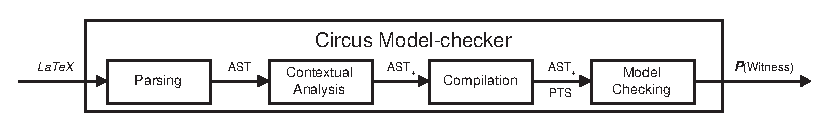
\epsfig{clip=, scale=0.9, file=mc.arch.stages.eps}
    \end{center}    \caption{\Circus\ Model Checking Stages}\label{mc-stages}
    \end{figure}
    %
    The theorem proving module present both in the compiler and refinement engine dispatches requests
    for evaluation of Z expressions and predicates as verification conditions over the state operations
    defined in Z, or possible enabling paths available for investigation from the behavioural actions
    given using CSP.
    At this point theorem proving is usually necessary to discharge proof obligations, and simplify
    expressions or predicates. Nevertheless, specifications have simple state operations, animation
    is also a good idea that can improve the automation of the model checking process.

    The role ZLive plays in this architecture is to tackle the requests to evaluate
    Z expressions and predicates from the compiler and refinement engine.
    As the operational semantics of \Circus\ is given in Z itself, we can use ZLive as a
    meta-level animator for simple specifications, hence enabling automatic model checking
    of state-rich \Circus\ specifications.
    With few improvements and extensions to the current implementation of ZLive to handle
    more of the schema calculus, we expect this to be a good example of how to integrate
    different CZT tools across different paradigms and boundaries.
    As the theorem proving integration architecture of the model checker allows pluggable
    solutions suitable for individual contexts, if ZLive cannot handle some complex \Circus\
    specifications, we can still resort to some alternative solution such as SAT solvers,
    and theorem provers.

\section{Section Manager}
\label{section-manager}

  [TODO: make this section nicer]

  Most of the tools mentioned in the previous sections use the section
  manager to enquire about specific aspects of a specification.  The
  section manager caches information about all the specifications and
  Z sections that are being processed;~records dependencies between
  them;~finds imported sections and toolkits;~automatically runs tools
  such as markup converters, parsers and typecheckers when necessary;~and
  is extensible to support user-defined commands.

  The CZT section manager can store any kind of data and is therefore
  independent of the Z extension used.  The cache is basically a mapping
  from a key to the actual data.  The key is a pair of a string,
  usually the name of the section, and a description of the type of
  data cached under this key.  For example, the Z parser adds the AST
  representation of a specification it has parsed to the section
  manager.  The type of a Z section in Java is
  \Interface{ZSect.class}, thus the AST for a section called foo is
  cached under the key \texttt{(``foo'',~ZSect.class)}.

  The default commands of the section manager are responsible to
  automatically compute requested data about sections. For example, if
  the AST (i.e. data of type \Interface{ZSect.class}) for section foo
  is required and has not already been cached, the Z parser is called
  by the section manager in order to parse the specification file
  containing section foo.  Here, the Z parser is the default command
  to compute data of type \Interface{ZSect.class}.

  When working with different Z extensions, a different
  parser might be required to parse specification documents.  The
  section manager can be reconfigured to use a different default
  command to compute data of type \Interface{ZSect.class}.  For
  example, the section manager can be configured to always use the
  Object Z parser.

\section{Other Tools}
\label{other-tools}

[LEO: Shall we mention the zpatt package here?]

\subsection{Testing Suites}

testing facilities (and test cases performed) in the CZT

\subsection{Converters}

z2b, zml2xhtml

\subsection{Available Front-Ends}

jedit, beanshell

\section{Conclusions and Future Work} \label{sec:conclusions}

\subsection{\Circus\ to JCSP}

        There is another tool under development that translates \Circus\ (Latex) specifications into Java code.
        It uses JCSP (a java csp-occam library) that allows execution of \Circus.
        In the Z part, due to the lack of tools, extreme simplifications (via data refinement in the original \Circus)
        are needed.
        This tool could also use ZLive to be able to animate/execute (run!) more expressive \Circus\ specifications quite
        automatically, or at least minimise the data refinement effort required for the translation.


\section*{Acknowledgements}

\bibliographystyle{splncs}
\bibliography{ifm}

\end{document}
